\documentclass[11pt, oneside]{article}   	% use "amsart" instead of "article" for AMSLaTeX format
\usepackage[margin = 1in]{geometry}                		% See geometry.pdf to learn the layout options. There are lots.
\geometry{letterpaper}                   		% ... or a4paper or a5paper or ... 
%\geometry{landscape}                		% Activate for rotated page geometry
\usepackage[parfill]{parskip}    		% Activate to begin paragraphs with an empty line rather than an indent
\usepackage{graphicx, ulem, tikz, multicol}				% Use pdf, png, jpg, or eps§ with pdflatex; use eps in DVI mode
								% TeX will automatically convert eps --> pdf in pdflatex		
\usepackage{amssymb, enumerate}

%SetFonts

%SetFonts


\title{Math F113X: Homework Set 6}
%\author{The Author}
\date{}							% Activate to display a given date or no date

\begin{document}
\maketitle
%\section{}
%\subsection{}

%Homework assignment 1 is:
%\vspace{-1.5cm}


\fbox{\parbox{\textwidth}{

Answer the following problems from the Graph Theory section \emph{in the order assigned.}\\

\begin{itemize} 
\item problems on Euler circuits, paths, eulerization:  A, 2, 14, 30, 32, 35a\\
\item problems on Hamiltonian circuits and paths: B, C, D, 17, 18\\
 \end{itemize}

}}

\quad\\

\textbf{Problem A:} For each graph below, (i) determine if it has an Euler circuit and (ii) determine if it has an Euler path. Justify your answer. \\

\begin{multicols}{3}
Graph $B_1$\\
\fbox{
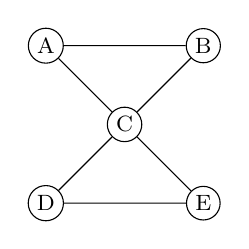
\begin{tikzpicture}
\tikzstyle{vtx}=[circle, draw, fill=black!0,
                        inner sep=1.5pt, minimum width=10pt, font = \footnotesize]
	\node[vtx] (A) at (-1,1){A};
	\node[vtx] (B) at (1,1){B};
	\node[vtx] (C) at (0,0){C};
	\node[vtx] (D) at (-1,-1){D};
	\node[vtx] (E) at (1,-1){E};
\draw (A)--(B)--(C)--(D)--(E)--(C)--(A);
\end{tikzpicture}
}

\columnbreak

Graph $B_2$\\
\fbox{
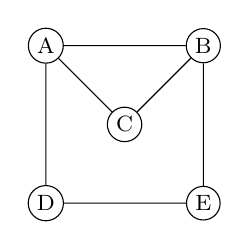
\begin{tikzpicture}
\tikzstyle{vtx}=[circle, draw, fill=black!0,
                        inner sep=1.5pt, minimum width=10pt, font = \footnotesize]
	\node[vtx] (A) at (-1,1){A};
	\node[vtx] (B) at (1,1){B};
	\node[vtx] (C) at (0,0){C};
	\node[vtx] (D) at (-1,-1){D};
	\node[vtx] (E) at (1,-1){E};
\draw (A)--(B)--(C)(B)--(E)--(D)--(A)--(C);
\end{tikzpicture}
}
\columnbreak

Graph $B_3$\\
\fbox{
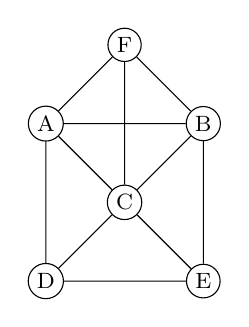
\begin{tikzpicture}
\tikzstyle{vtx}=[circle, draw, fill=black!0,
                        inner sep=1.5pt, minimum width=10pt, font = \footnotesize]
	\node[vtx] (A) at (-1,1){A};
	\node[vtx] (B) at (1,1){B};
	\node[vtx] (C) at (0,0){C};
	\node[vtx] (D) at (-1,-1){D};
	\node[vtx] (E) at (1,-1){E};
	\node[vtx] (f) at (0,2){F};
\draw (A)--(B)--(C)--(D)--(E)--(C)--(A)--(D)(E)--(B);
\draw (A)--(f)--(B)(C)--(f);
\end{tikzpicture}
}
\end{multicols}

\hrulefill

\textbf{Problem B:} 
\begin{enumerate}
\item Write out what $5!$ means and find its value.
\item Expand $8.75 \times 10^8$
\item Write $35,200,000$ in scientific notation.
\item Use any computational device to compute $20!$ and write it in scientific notation, holding only the first three digits.\\
\end{enumerate}

\hrulefill
\vfill

\textbf{Problem C:} This question is about \textbf{complete graphs} and \textbf{complete bipartite graphs}.\\
A complete graph on $n$ vertices is the graph that includes an edge between every pair of distinct vertices, denoted $K_n.$ A complete balanced bipartite graph on $2n$ vertices, denoted $K_{n,n}$, is the graph that splits the vertex set into two equal sets and includes every edge between the two sets. Examples are below.

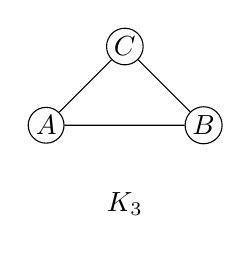
\begin{tikzpicture}
\node[circle, draw,  inner sep=1pt] (a) at (-1,0){$A$};
\node[circle, draw,  inner sep=1pt]  (b) at (1,0){$B$};
\node[circle, draw,  inner sep=1pt]  (c) at (0,1){$C$};
\node at (0,-1){$K_3$};
\draw (a) -- (b)--(c) --(a);
\end{tikzpicture}
\hfill
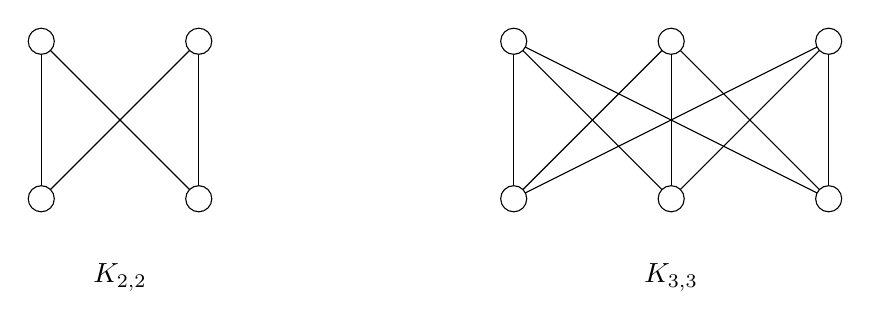
\begin{tikzpicture}
\tikzstyle{vtx}=[circle, draw, fill=white,minimum size=2pt]
\node at (1, -1){$K_{2,2}$};
\node at (8,-1){$K_{3,3}$};
\tikzstyle{every node} = [vtx];
\foreach \i in {6,8,10}{
	\draw (6,0) -- (\i,2);
	\draw (8,0) -- (\i,2);
	\draw (10,0) -- (\i,2);}
\foreach \i in {0,2}{
	\draw (0,0) -- (\i,2);
	\draw (2,0) -- (\i,2);}
\foreach \i in {0,2,6,8,10}{
	\node  at (\i,0){};
	\node at (\i,2){};}
\end{tikzpicture}

 
	\begin{enumerate}
	\item Draw $K_4,$ $K_5,$ and $K_6.$
	\item Draw $K_{4,4}.$
	\item How many edges would $K_{10}$ have? How many edges would $K_{10,10}$ have?
	\item Give an example of a practical situation that could be modeled by a weighted $K_{10,10}$? (State what the vertices and edge weights represent.)\\
	\end{enumerate}
	
\hrulefill
	\vfill
	
\textbf{Problem D:} Answer the questions about the graph below.
\begin{center}
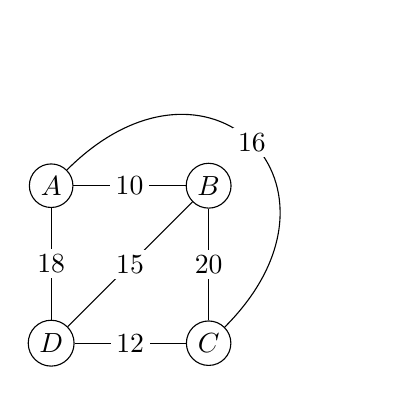
\begin{tikzpicture}[lbl/.style={inner sep = 2pt, fill = white}]
\tikzstyle{vtx}=[circle, draw, inner sep=2pt]
\node[vtx] (A) at (0,2){$A$};
\node[vtx] (B) at (2,2){$B$};
\node[vtx] (C) at (2,0){$C$};
\node[vtx] (D) at (0,0){$D$};
\foreach \i/\j/\k in {A/B/10,B/C/20,C/D/12,D/A/18,B/D/15}{\draw (\i) --node[lbl]{\k} (\j);}
\draw (A) .. controls (2,4) and (4,2) .. (C)
  node[pos=0.5,inner sep = 2pt, fill = white]{$16$};
\end{tikzpicture}
\end{center}

\begin{enumerate}
\item List all of Hamiltonian circuits and calculate their weight.
\item Using the list above, identify a circuit with the lowest total weight.
\item The steps above are those of what algorithm?
\item Find a Hamiltonian \emph{path} of lowest total weight, and justify your conclusion.
\end{enumerate}


\hrulefill

Remember to write up your homework solutions according to the homework writeup guidelines. 

Homework is graded using the following rubric for each problem (or problem part):

\begin{description}
\item[2 points:] You provided a complete answer, with supporting work, written up clearly
\item[1 point:] Some attempt at a solution, but incomplete writeup / unclear / illegible / no answer
\item[1 point:] Only an answer, with no supporting work 
\item[0 points:] Missing.
\end{description}

After you do the homework, you need to check your answers against the solutions! Then figure out your errors (if any) and revise your homework before you submit it. 

Homework must be submitted on Gradescope.

\end{document}  